\documentclass[10pt]{beamer}
\usepackage{pgfpages}
\usepackage[utf8]{inputenc}
\setbeameroption{show notes}
%\setbeameroption{show notes on second screen}


\usetheme[progressbar=frametitle]{metropolis}
\usepackage{appendixnumberbeamer}

\usepackage{booktabs}
%\usepackage[scale=2]{ccicons}

%\usepackage{pgfplots}
%\usepgfplotslibrary{dateplot}

%\usepackage{xspace}
%\newcommand{\themename}{\textbf{\textsc{metropolis}}\xspace}

\usepackage{lipsum}

\usepackage{tikz}
\usetikzlibrary{positioning, arrows, shapes}
\usetikzlibrary{shapes}
% Define box and box title style
\tikzstyle{mybox} = [draw, very thick, rectangle, inner sep=10pt, inner ysep=20pt, fill=black, text=white, minimum width=\textwidth, minimum height=2cm]

\tikzstyle{redRectangle} = [
    rectangle,
    draw,
    fill=red!20,
    node distance=0.85 cm,
    text width=7 em,
    text centered,
    rounded corners,
    minimum height=4 em,
    minimum width=3 cm,
    thick
    ]
    \tikzstyle{blueRectangle} = [
    rectangle,
    draw,
    fill=blue!20,
    node distance=1.5 cm,
    text width=7 em,
    text centered,
    rounded corners,
    minimum height=4 em,
    minimum width=3 cm,
    thick
    ]
    \tikzstyle{yellowRectangle} = [
    rectangle,
    draw,
    fill=yellow!20,
    node distance=1.5 cm,
    text width=7 em,
    text centered,
    rounded corners,
    minimum height=4 em,
    minimum width=3 cm,
    thick
]
\tikzstyle{empty} = []

%Telling a story with your code: Literate Programming with Notebooks
%The ideas of provenance, scientific workflow and reproducibility are key to the development of good scientific code. In this talk, we explore the fundamentals of Literate Programming, an idea that has been around for decades but has had surprisingly little influence in most disciplines. Of course, the idea of Notebooks is heavily based on this concept. We discuss how telling a story with your code – not only showing your results, but how you got there – can be an invaluable tool in teaching and research, and most of all in sharing your results with other researchers and colleagues. Brief examples will be shown using Jupyter Notebooks.

\title{Telling a story with your code}
\subtitle{Literate Programming with Notebooks}
% \date{\today}
\date{RSE2017}
\author{Melissa Weber Mendonça}
\institute{UFSC}
\titlegraphic{\hfill\includegraphics[height=1.5cm]{brasao_UFSC.png}}

\begin{document}

\maketitle

\begin{frame}
  \frametitle{Motivation}
  \begin{center}
    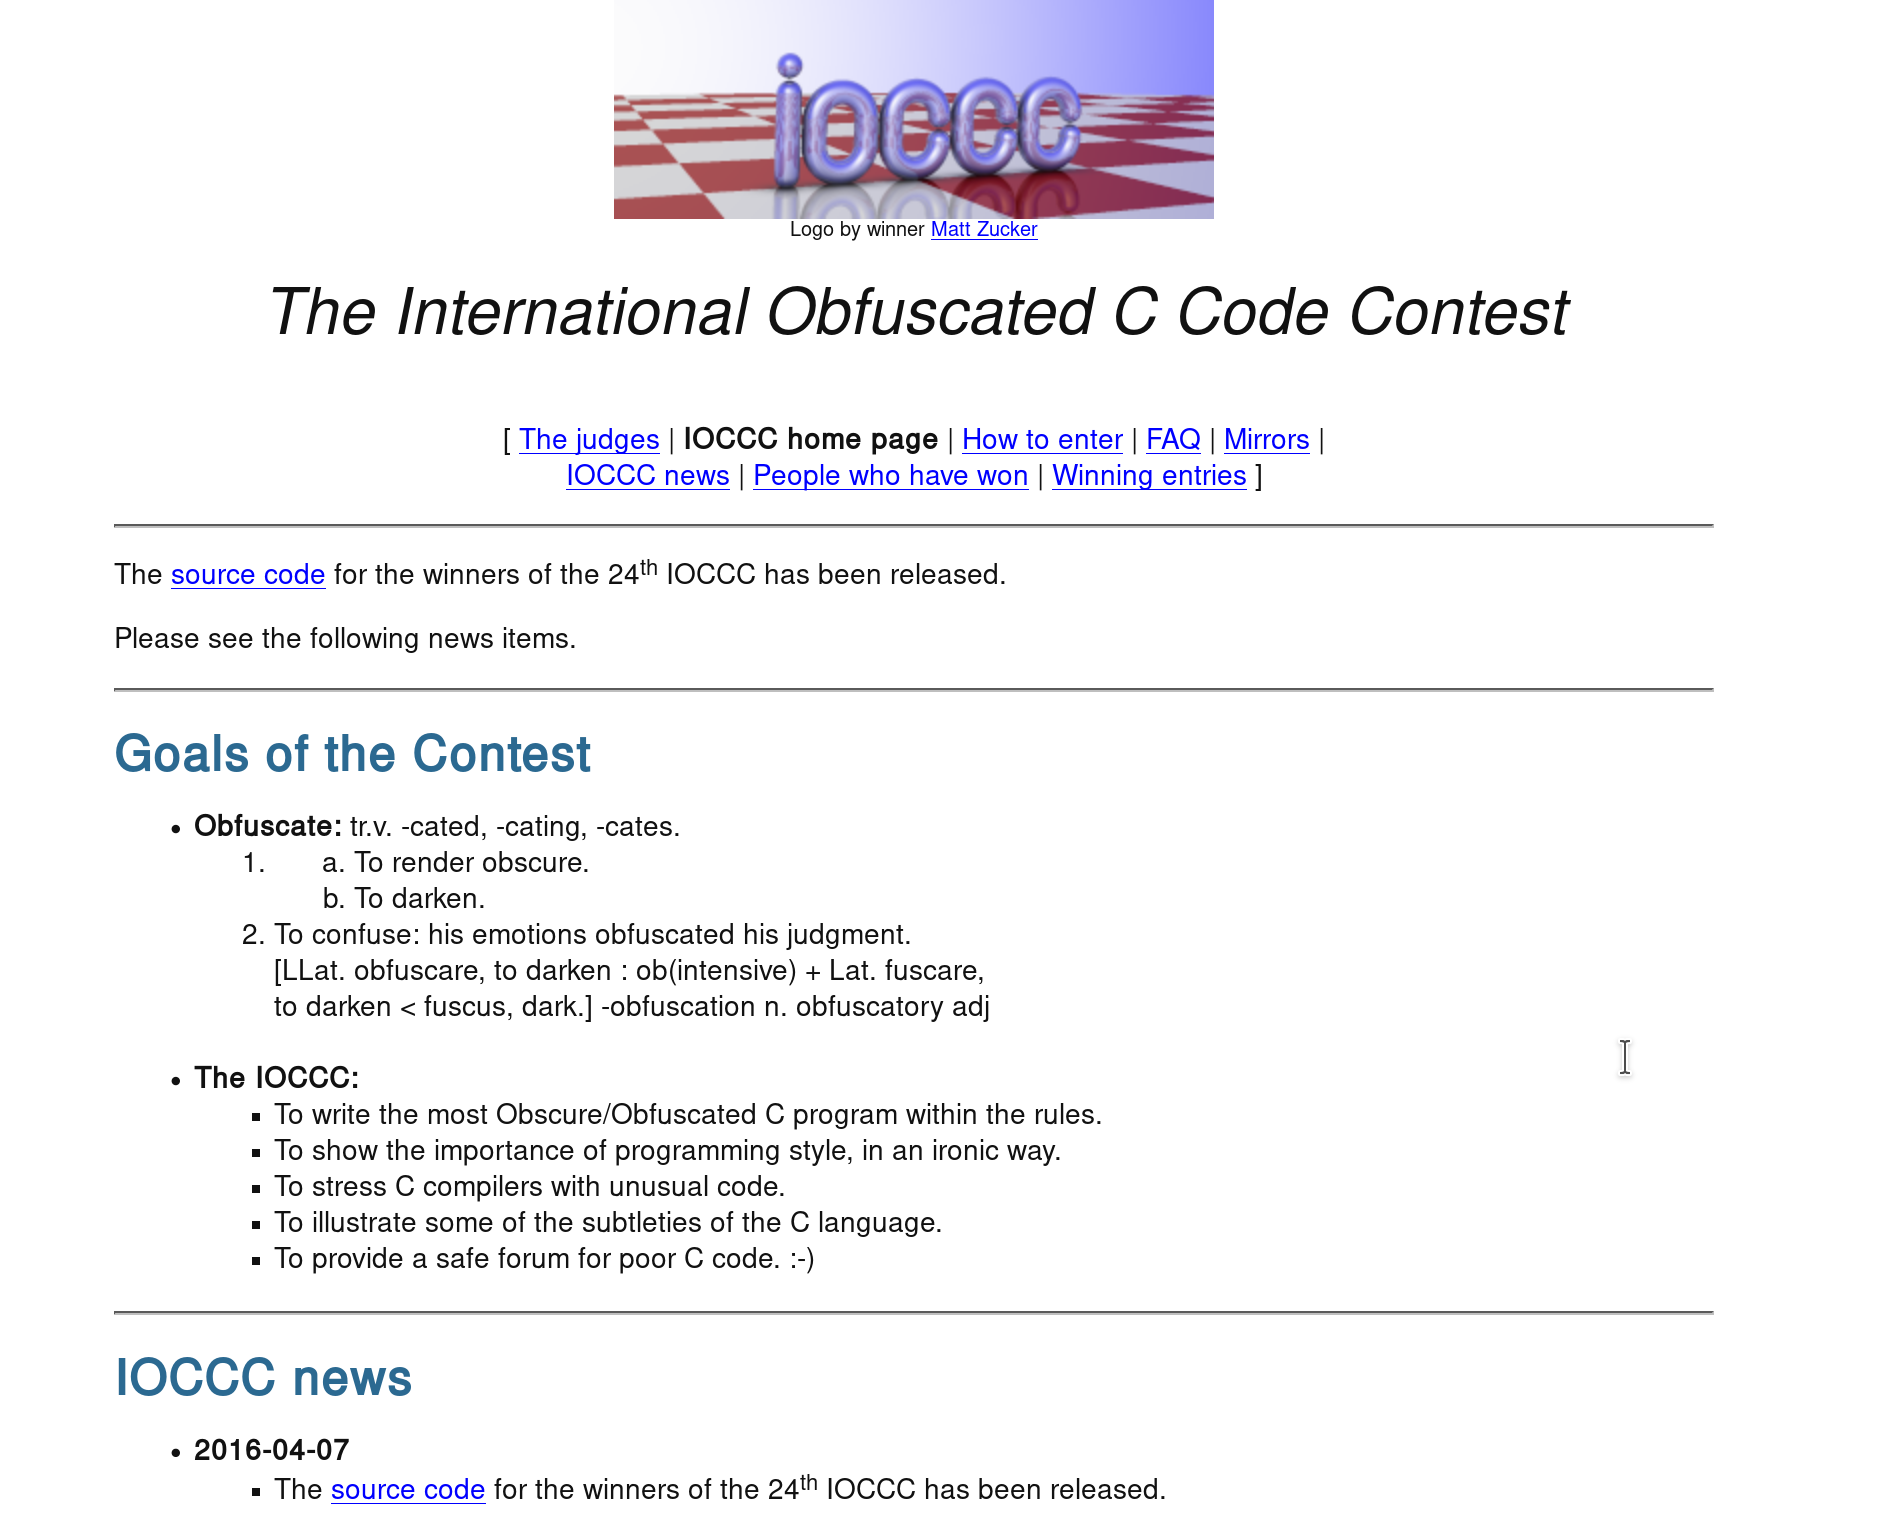
\includegraphics[width=0.9\textwidth]{obfuscated.png}
  \end{center}
  \note{Our main motivation is something like this. I don't know if you've heard of this contest. Basically, people are competing to see who writes the most obfuscated code, the less legible one.}
\end{frame}

\begin{frame}
  \frametitle{Motivation}
  \begin{center}
    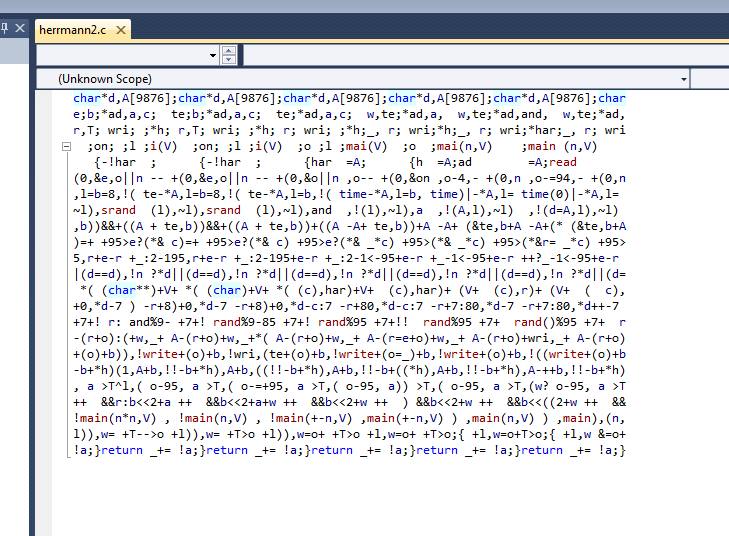
\includegraphics[width=0.9\textwidth]{ioccc.png}
  \end{center}
  \note{Unfortunately, most of the code we (at least for me) are used to reading is something that could be in this contest, in whatever language (especially MATLAB). It is easy for researchers and students to copy and paste code from everywhere around the internet or from legacy projects and never question how or WHY they work. My PhD advisor, Philippe Toint, used to say that code should be written and read like liteature; that you can learn how to write good code by reading good code. That a program should ideally be read like a scientific article. It took me a long time to really understand what he meant, but when I read about literate programming, I knew this is what he was talking about.}
\end{frame}

\begin{frame}
  \frametitle{Literate Programming}
  \begin{center}
    \begin{columns}[totalwidth=11cm]
      \begin{column}{0.65\textwidth}
        \textbf{Donald Knuth, \emph{Literate Programming} (1984)}\\
        % \footnote{in Literate Programming. CSLI, 1992, pg. 99.}}
        ``Let us change our traditional attitude to the construction of programs: Instead of imagining that our main task is to instruct a computer what to do, let us concentrate rather on explaining to human beings what we want a computer to do.       

        The practitioner of literate programming can be regarded as an essayist, whose main concern is with exposition and excellence of style. Such an author, with thesaurus in hand, chooses the names of variables carefully and explains what each variable means.''
      \end{column}

      \begin{column}{0.35\textwidth}
        \begin{center}
          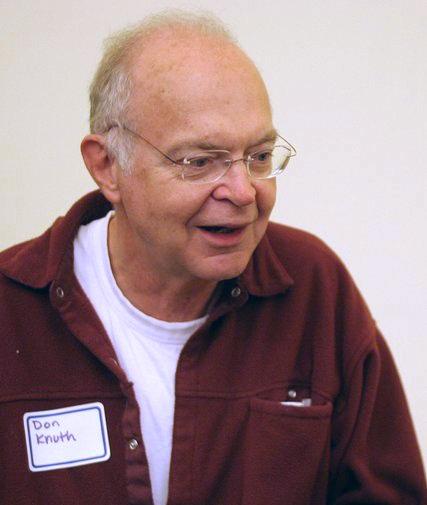
\includegraphics[width=2.5cm]{knuth.jpg}\\
          Don Knuth
        \end{center}
      \end{column}
    \end{columns}
  \end{center}

  \note{Enter Don Knuth. I'm sure you've heard of him before. In 1981 he thought about these things because he disagreed that structured programming was necessarily the way to go forward. In fact, he thought programming following the computer logic was a bad way to write code. He created the idead of Literate Programming based on this idea: "Instead of imagining that our main task is to instruct a computer what to do, let us concentrate rather on explaining to human beings what we want a computer to do." }  
\end{frame}

\begin{frame}
  \frametitle{Ideas}
  \begin{itemize}
  \item<1-> Code as \alert{literature}
  \item<2-> Explicitly describing your reasoning
  \item<3-> Better documentation
  \end{itemize}

  \note{\footnotesize{So there are some interesting points we can make.
    \begin{itemize}
    \item The first idea is to recognize ``code as literature''. Not only should we be able to read good code and learn from it, our code should tell a story: we should describe not only \alert{how} we are solving the problem at hand, but we should describe \alert{why} we are solving it that way. 
    \item This is the second point: ``Explicitly describing your reasoning''. Someone reading our code should be able to detect why we chose this implementation, why this is the appropriate method, why did we choose a while instead of choosing a for. After all, if your code is reasonable, it should not be so difficult to understand what is being done.
    \item But more than this, the idea of literate programming is also to provide an organic documentation, meaning that code and documentation are linked in such a way that it's impossible to lose compatibility or to change the code without changing the documentation.
    \end{itemize}}
  }
\end{frame}

\begin{frame}[fragile]
  \frametitle{Literate Programming in practice: WEB}
  WEB [https://en.wikipedia.org/wiki/WEB]

  \begin{itemize}
  \item Natural Language + macros/code
  \item \emph{Compilable}
  \item Code can be \emph{nonlinear}
  \end{itemize}

  \begin{center}
    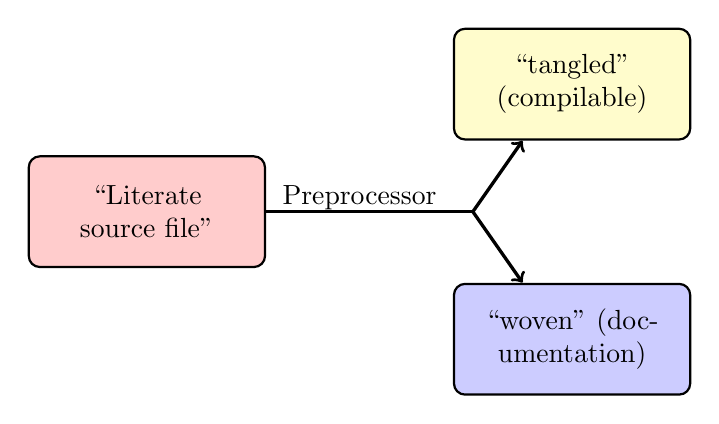
\begin{tikzpicture}[scale=0.9]
      \node[redRectangle] at (0,0) (source) {``Literate source file''};
      \draw[very thick] (source.east) -- (4.6,0);
      \node[] at (3,0.2) {Preprocessor};
      \draw[very thick, ->] (4.6,0) -- (5.3,1);
      \draw[very thick, ->] (4.6,0) -- (5.3,-1);
      \node[yellowRectangle] at (6,1.8) {``tangled'' (compilable)};
      \node[blueRectangle] at (6,-1.8) {``woven'' (documentation)};
    \end{tikzpicture}
  \end{center}

  \begin{center}
    \href{https://github.com/zyedidia/Literate/blob/master/examples/wc.lit}{\beamergotobutton{wc.lit}}
  \end{center}

  \note{web is a combination of two languages: a Document formatting Language and Programming language. Initially, the idea was to use Pascal and TeX, but there are other options. The main characteristic is to mix natural language with code and or macros, that there is only one final compilable document, and code can be written in a nonlinear way, that is, we can cross reference other sections or procedures in the document so that the document does not have to be written in the order the machine expects.}
\end{frame}

\begin{frame}
  \frametitle{Other ideas for implementation}
  \begin{itemize}
  \item WEB \textemdash\ Pascal + \TeX\ (Knuth) 
  \item CWEB \textemdash\ C + \TeX\ (Knuth and Silvio Levy)
  \item Sweave \textemdash\ R + \TeX
  \item knitr \textemdash\ R+\TeX
  \item noweb \textemdash\ Language? + Format? (HTML)
  \item iJulia
  \item Pweave \textemdash\ Python + Format? (Pandoc)
  \item \alert{iPython/Notebooks}
  \end{itemize}
  \note{There are several tools that can do literate programming.}
\end{frame}

\begin{frame}
  \frametitle{What is \emph{not} Literate Programming}
  \begin{itemize}
  \item Well documented code
  \item Reports mixing code and text 
  \item Automatic documentation
  \item Notebooks written in a ``traditional'' format (pasting code into a notebook instead of using an IDE)
  \end{itemize}
  \note{Just writing good documentation or doing reports mixing code and text are not examples of LP. Just having a bunch of text and a bunch of code does not necessarily link them, and does not necessarily help explain why those choices were made, or why the code worksthe way it does.}
\end{frame}

\begin{frame}
  \frametitle{How can this help us?}

  \begin{itemize}
  \item[1.]<1-> Communication
    \begin{itemize}
    \item Research
    \item Teaching
    \end{itemize}
    
  \item[2.]<2->Research and reproducibility: how did we get here?
    \begin{itemize}
    \item Provenance
    \item Scientific workflow
    \end{itemize}
  \end{itemize}

  \note{Explain how we got here; which mistakes were made, bad assumptions, bad methods, WHY}
\end{frame}


\begin{frame}[fragile]
  \frametitle{Examples}
     \begin{center}
      \begin{minipage}{0.7\textwidth}
      \begin{block}{}
         \begin{center}
              \verb+IDEB.ipynb+
         \end{center}
      \end{block}
    \end{minipage}
   \end{center}
   \vfill
   A few useful tools:
   \begin{itemize}
   \item \LaTeX; Pandoc
   \item nbextensions: codefolding, initialization cell, limit output
   \item Preprocessors and templates for notebooks: automatic documentation
   \end{itemize}

   \note{Open example}
\end{frame}

\begin{frame}[fragile]
   \frametitle{Let's talk about it!}
   \begin{center}
      \begin{minipage}{0.7\textwidth}
      \begin{block}{}
         \begin{center}
           \verb+github.com/melissawm+\\
           \verb+github.com/melissawm/rse2017+\\
            \verb+www.mtm.ufsc.br/~melissa+\\
            \verb+melissawm@gmail.com+
         \end{center}
      \end{block}
    \end{minipage}
    \vfill
  \end{center}

  \note{ Thank you.}
\end{frame}

\begin{frame}[allowframebreaks, fragile]{Supporting Material}

  Fernando Pérez's blog post on Literate Computing: from 2013! \href{http://blog.fperez.org/2013/04/literate-computing-and-computational.html}{\alert{[link]}}
  
  \begin{itemize}
  \item Good notebooks:
    \begin{itemize}
    \item \href{http://nbviewer.jupyter.org/gist/rpmuller/5920182}{A Crash Course in Python for Scientists (Rick Muller)}
    \item \href{http://nbviewer.jupyter.org/github/jrjohansson/scientific-python-lectures/blob/master/Lecture-4-Matplotlib.ipynb}{matplotlib \textemdash\ 2D and 3D plotting in Python (J.R. Johansson)}
    \end{itemize}
  \item Bad notebooks:
    \begin{itemize}
    \item \href{http://nbviewer.jupyter.org/github/facebook/iTorch/blob/master/iTorch_Demo.ipynb}{iTorch Demo (??)}
    \item \href{http://nbviewer.jupyter.org/github/rasbt/pattern_classification/blob/master/data_viz/swapi_viz.ipynb}{Star Wars API}
    \end{itemize}
  \end{itemize}
  % Link interessante!
  % http://blog.juliusschulz.de/blog/ultimate-ipython-notebook
\end{frame}
\end{document}